% \begin{anexosenv}

% % Imprime uma página indicando o início dos anexos
% \partanexos

% % Para cada anexo, um \chapter


% %==============================================================================
% \chapter{Primeiro Anexo}
% %==============================================================================

% Sendo anexo, a formatação dessa seção é livre. Ou seja: aceita-se fonte diferente e menor


% %==============================================================================
% \chapter{LaTex para Principiantes}\label{anexo:latex}
% %==============================================================================
% TEste\footnote{\cite{Moro2012}}
% Dentro dos arquivos .tex o texto pode estar organizado em partes, capítulos, seções, etc. conforme os seguintes comandos:

% -- \verb|\part{NomedaParte}|, partes do documento \\
% -- \verb|\chapter{Nome}|, capítulos somente para arquivos do tipo \textit{book} e \textit{report}\\
% -- \verb|\section{Nome}|, seções\\
% -- \verb|\subsection{Nome}|, subseções	\\
% -- \verb|\subsubsection{Nome}|, seções dentro de subseções\\
% -- \verb|\paragraph{Texto}|, parágrafos formatados	\\
% -- \verb|\subparagraph{Texto}|, subparágrafos

% \textbf{Parágrafos} Parágrafos são definidos deixando uma linha em branco entre os mesmos.
%   Pode-se também forçar usando \verb|\\| bem como deixar uma linha em branco com um \verb|~| sozinho na linha.

% \textbf{Formato de texto} O tamanho do texto pode ser definido pelos comandos específicos:  \verb|tiny|,  \verb|scriptsize|,  \verb|footnotesize|, \verb|small|, \verb|normalsize|, \verb|large|, \verb|Large|, \verb|huge| e \verb|Huge|, conforme ilustra a Figura \ref{fig:fontsize}\todo{Perceba que a figura tem resolução ruim; deveria ser uma tabela}.

% \begin{figure}[ht]
% 	\centering
% 		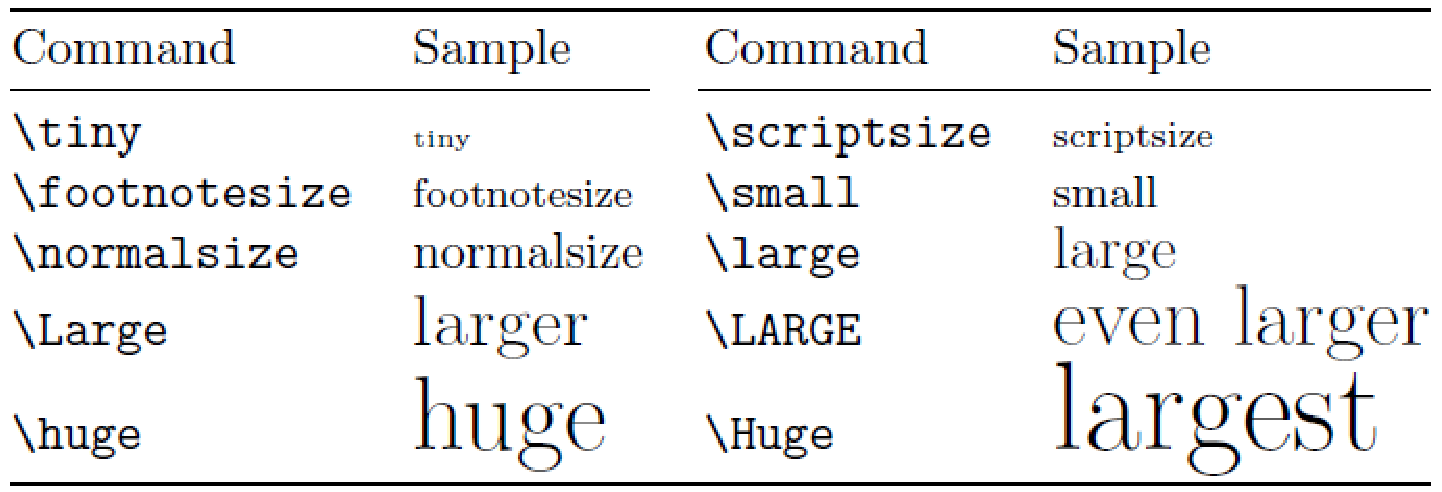
\includegraphics[width=0.7\textwidth]{img/fontsize}
% 	\caption{Exemplo de tamanhos de fonte}
% 	\label{fig:fontsize}
% \end{figure}

% \textbf{Referências dentro do Texto} Partes do texto podem ser referenciadas através do par de comandos \verb|\label| e \verb|\ref|.
%   Por exemplo, podemos inserir uma seção no artigo utilizando o seguinte comando:

% \begin{verbatim}
% \section{Seção principal}\label{sec:prcpal}
% \end{verbatim}

% Vejam que o título da seção é seguido do comando \verb|\label{nome}|.
%   Esta seção pode ser referenciada em qualquer parte do texto, como o exemplo a seguir.

% \begin{verbatim}
% Conforme explicado na Seção \ref{sec:prcpal}, nosso método utiliza...
% \end{verbatim}


% %------------------------------------------------------------------------------
% \section{Outras Dicas}
% %------------------------------------------------------------------------------

% \textbf{Caracteres Especiais} Esses não podem ser usados no texto sem a barra à frente: \# \$ \% \^{ } \& \_ \{ \} \~{ } e \slash .

% \textbf{Comentários} Comentários são precedidos de \% e podem estar em qualquer parte do texto.
%   Lembrando que tudo que estiver após \% será considerado como comentário e ignorado pelo processador.

% \textbf{Incluir Figuras} Incluir figuras no LaTeX é relativamente fácil quando se tem um formato de arquivo pré-definido.
%   or exemplo, neste documento, usa-se apenas figuras do tipo \textit{pdf}, mas também poderia-se usar do tipo \textit{png} (e \textit{jpeg}, mas este tipo não é recomendado).
%   A Tabela \ref{tab:codfig} ilustra as linhas que inserem uma figura no texto. 

% \begin{table}[!htb][ht]
%   \caption{Linhas de código para inserir figura}
% 	\centering
% 	\footnotesize	
% 		\begin{tabular}{l l}
% 	\\	\hline 
% Linha de Código & Explicação \\ \hline 
% \verb|\usepackage{graphicx}| & \textit{inclui pacote gráfico no início do documento} \\
% \verb|\begin{figure}[tb]|    & \textit{inicia figura, define sua posição no texto} \\
% \verb|\centering|            & \textit{centraliza a figura na página}\\
% \verb|\includegraphics[scale=.7]|& \textit{define escala da figura}\\
% \verb|{img/figura}|      & \textit{inclui o arquivo da figura no texto}\\
% \verb|\caption{Legenda}|     & \textit{inclui a legenda da figura}\\
% \verb|\label{fig:ap}|        & \textit{inclui o apelido da figura}\\
% \verb|\end{figure}|          & \textit{termina figura}\\
% 		\hline\end{tabular}
% 	\label{tab:codfig}
% \end{table}

% \textbf{Hifenização} Às vezes aparece uma palavra cuja hifenização, divisão silábica, está errada. Para resolver esse tipo de problema, pode-se recorrer à divisão manual da palavra, acrescentando \verb|\-| entre cada sílaba: \verb|Mi\-re\-lla|. Se, ao invés desta solução, você quiser evitar completamente que suas palavras sejam divididas, acrescente os dois comandos no início do seu documento (ou seja, antes do \\~\textit{begin\{document\}}).

% \begin{verbatim}
%   \hyphenpenalty=5000
%   \tolerance=1000
% \end{verbatim}


% \textbf{BibTeX} Para editar facilmente o BibTeX, pode-se utilizar uma ferramenta própria\footnote{Ferramentas para BibTeX: http://dmoz.org/Computers/Software/Typesetting/TeX/BibTeX}. A minha favorita é o JabRef\footnote{JabRef Editor: http://jabref.sourceforge.net/}, ilustrado na Figure \ref{fig:jabref}, porque:

% \begin{itemize}\addtolength{\itemsep}{-0.5\baselineskip}
% 	\item É de graça;
% 	\item Possui interface gráfica super intuitiva;
% 	\item Permite importar referências de bases clássicas, como ISI, Medline e RIS;
% 	\item Permite exportar para diferentes formatos, inclusive para um banco de dados utilizando SQL;
% 	\item Tem botão para procurar o artigo da respectiva referência e fazer o seu download;
% 	\item Permite adicionar comentários próprios para cada entrada;
% 	\item Pode-ser classificar as referências e criar grupos para as mesmas, e muito muito mais.
% \end{itemize}

% \begin{figure}[tb]
% 	\centering
% 		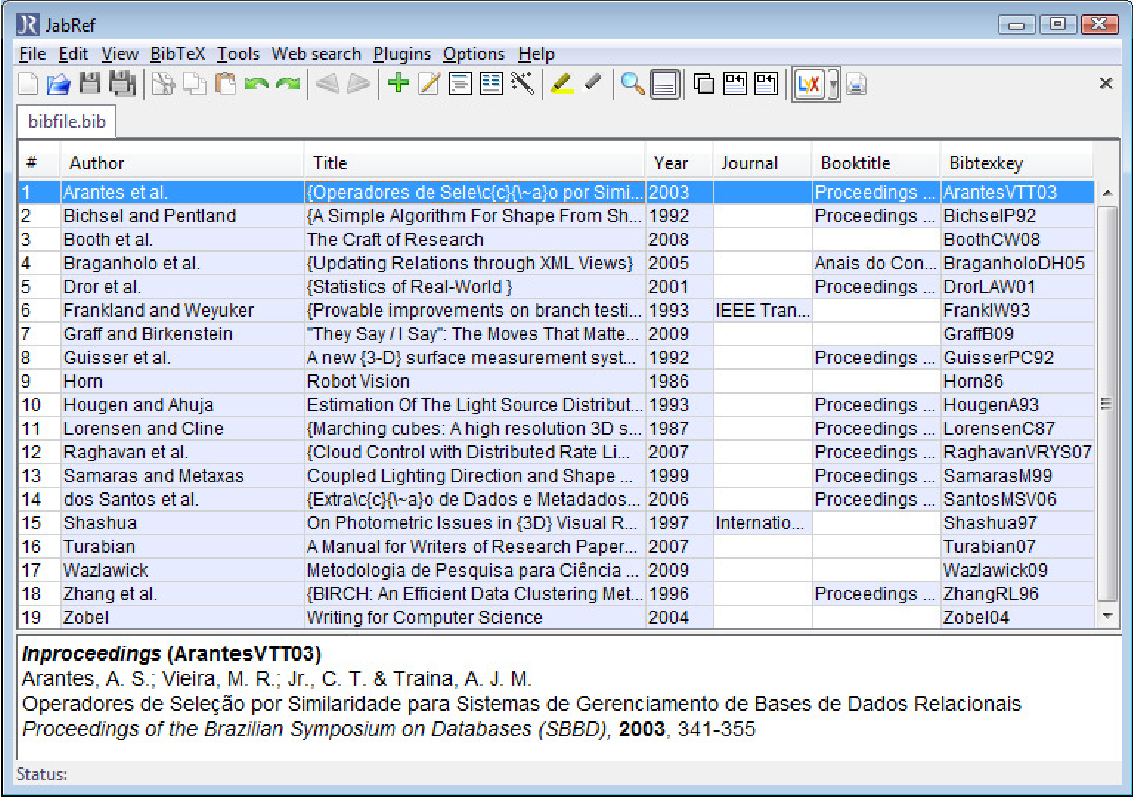
\includegraphics[width=0.98\textwidth]{img/jabref}
% 	\caption{Tela do JabRef para uma versão inicial do arquivo bib deste documento}
% 	\label{fig:jabref}
% \end{figure}

% \textbf{Listas} Listas podem ser definidas com \textit{bullets} ou com números, conforme os exemplos a seguir.

% \begin{verbatim}
% \begin{itemize}
% \item Item 1 com bullet 
% \item Item 2 com bullet 
% \end{itemize}

% \begin{enumerate}
% 	\item Item 1 numerado
% 	\item Item 2 numerado
% \end{enumerate}
% \end{verbatim}

% \textbf{Fontes Coloridas} Para adicionar texto em cores (muito útil para marcar trechos do texto que estão \textit{em trabalho}, deve-se adicionar os pacotes \textit{graphicx} e \textit{color} (usando o comando \verb|\usepackage| e depois utilizar o comando \verb|\textcolor{cor}{texto}| para colorir o \textit{texto} com a \textit{cor} especificada. Por exemplo \verb|\textcolor{blue}{texto em azul}|. Outras cores comuns são \textit{red} e \textit{green}.

% \textbf{Para Economizar Espaço} Existem alguns \textit{dirty tricks}\footnote{Ou seja, eles irão alterar a formatação dada pelo estilo default do texto.} pra economizar espaço, como por exemplo:

% -- \verb|\usepackage{times}| Usa fonte \textit{Times} no lugar da default.

% -- \verb|\usepackage[small,compact]{titlesec}| Modifica o título e os espaços antes/depois dos mesmos.

% -- \verb|\usepackage[small,it]{caption}| Reduz o tamanho das legendas de tabelas e figuras.

% \textbf{WEB} A Web é repleta de páginas e documentos sobre LaTeX. Alguns exemplos incluem:

% \begin{itemize}\addtolength{\itemsep}{-0.5\baselineskip}
%   \item Favorito inglês: \url{http://en.wikibooks.org/wiki/LaTeX/}
%   \item Favorito português: \url{http://linorg.usp.br/CTAN/info/lshort/portuguese/pt-lshort.pdf}
%   \item \url{http://www.mat.ufmg.br/~regi/topicos/intlat.pdf}
%   \item \url{http://www.duke.edu/~hg9/ctex/LaTeXManual.pdf}
%   \item \url{http://minerva.ufpel.tche.br/~campani/cursolatex.pdf}
% 	\item \url{http://www.personal.ceu.hu/tex/words.htm}
% \end{itemize}


% \end{anexosenv}
